\scanpage{42}
Dual de $L_0(E,F)$. \deleted{\unsure{Cet}} \unsure{Mettons cet espace en dualité naturelle} avec $L^{(1)}(F,E)$, \deleted{\unsure{soit}} par
\[
\boxed{(u,v)=\operatorname{Tr}vu}
\]
(les $E'\otimes F$ et $F'\otimes E$, \unsure{cela comme on sait bien})
et l'application naturelle de $L^1(F,E)$ dans $(L_0(E,F))'$ est une isométrie : si $v\in L^1(F,E)$ et est $\sum\unsure{\rho_i|\lambda_i}\overline f_i\otimes e_i$, il suffit de prendre $u=\sum_1^n\unsure{\rho_i}\overline e_i\otimes f_i$ pour trouver $(u,v)=\sum_1^n\rho_i$.
Montrons qu'il est \uline{sur}. En effet, si $\varphi$ est une forme linéaire continue sur $L_0(E,F)$, alors $\varphi(x'\otimes y)$ est une forme bilinéaire continue sur $E'\times F$, donc définit une application linéaire $F\longrightarrow E$, \unsure{soit} le $v$. On a $\varphi(u)=\operatorname{Tr}vu$, il reste à montrer que $v$ est de Fredholm, sachant $|\operatorname{Tr}vu|\leq M\|u\|$ pour $u\in E'\otimes F$.

\deleted{Considérons $\unsure{w=vv^*}\in L(E,E)$, on a \deleted{$\unsure{\operatorname{Tr}uvv^*=\operatorname{Tr}v^*uv}$} \deleted{$u\in\unsure{L(E,E)}$} \unsure{$u\in E'\otimes E$}
\[
|\operatorname{Tr}uw|=|\operatorname{Tr}uvv^*|=|\operatorname{Tr}v^*uv|\leq M\|v^*u\|;
\]
donc $w$ a la même propriété que $v$. Or \deleted{\illegible{3}} \unsure{$w$ est encore un op.} compact (donc $v$ sera compact) :}

$w=(vv^*)^{1/2}\in L(E,E)$, alors $v=Ww$, $w=Vv$, on voit aussitôt que $w\inserted{{}=Vv}$ \deleted{\unsure{est}} vérifie \unsure{la propriété} de $v$, montrons que $w$ est op. de Fredholm, donc $v\inserted{{}=Ww}$ le sera (le \unsure{précédent} : $F=E$).
Or \deleted{\illegible{1}} d'abord $w$ est cpt, \unsure{car} autrement il \unsure{existerait} un sous espace $H\subset E$ \uline{\unsure{stble}} \inserted{stable} \uline{par} \inserted{sous} $w$, où $w$ serait inversible, ce qui amène une contradiction.
\margin{\figure{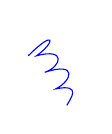
\begin{tikzpicture}[x=0.35cm,y=0.35cm]\draw[blue] (0,1.8) .. controls (1,2.8) and (1,2.3) .. (0.3,1.8) .. controls (1.4,2.1) and (1.2,1.4) .. (0.6,1.2) .. controls (1.8,1.6) and (1.6,0.9) .. (1,0.6) .. controls (2,0.8) and (1.5,0.2) .. (1.4,0);\end{tikzpicture}}}
On aura donc $w=\sum\rho_i\overline f_i\otimes e_i$, et prenant $u=\sum_1^n\overline e_i\otimes f_i$, on trouve
\[
\sum_1^n\rho_i\leq M.
\]
D'où la conclusion.
\margin{\figure{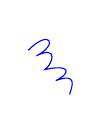
\begin{tikzpicture}[x=0.35cm,y=0.35cm]\draw[blue] (0,1.6) .. controls (0.8,2.4) and (1.1,1.8) .. (0.3,1.4) .. controls (1.1,1.8) and (0.9,1.1) .. (0.6,0.9) .. controls (1.5,1.1) and (1.6,0.8) .. (1,0.5) .. controls (1.8,0.8) and (1.6,0.3) .. (1.5,0);\end{tikzpicture}}}

--- \unsure{Méthode} \inserted{méthode} plus élémentaire : $\varphi$ est une forme linéaire continue sur $L^{\unsure{2}}(E,F)$, donc donnée par un $v\in L^2(F,E)$, qui est en particulier cpt. On achève comme tout à l'heure.
\mspage{43}
